\section{Integration von Statischer Code Analyse in den DevOps-Zyklus}
In diesem Kapitel wird anhand von statischer Code-Analyse und Dependency Scanning aufgezeigt, wie Sicherheitslücken erkannt und behoben werden können, bevor diese in für den Produktionsbetrieb freigegebenen Releases veröffentlicht und in Betrieb genommen werden.

\subsection{Nutzung von Statischer Code Analyse}
Die Nutzung von statischer Code-Analyse ist ein essenzieller Bestandteil moderner Softwareentwicklungsprozesse, um die Codequalität und Sicherheit zu gewährleisten. Es gibt eine Vielzahl von Tools zur Durchführung dieser Analysen, darunter SonarQube, ESLint, Pylint und Coverity. Die Autoren dieses Kapitels fokussieren sich auf die Verwendung von SonarQube, basierend auf ihrer umfangreichen Erfahrung und den Vorteilen, die SonarQube bietet. SonarQube wird häufig gewählt, weil es eine umfassende Analyse für eine Vielzahl von Programmiersprachen bietet und sich nahtlos in verschiedene CI/CD-Tools integrieren lässt.

Durch die Integration von SonarQube in den CI/CD-Prozess kann diese Analyse automatisiert und kontinuierlich durchgeführt werden. Innerhalb des GitFlow-Workflows ermöglicht es die Einrichtung von Quality Gates in SonarQube, die spezifische Richtlinien und Kriterien definieren, die der Code erfüllen muss. Wenn diese Quality Gates durch die in SonarQube hinterlegten Policies fehlschlagen, wird der Build-Prozess unterbrochen und ein Merge in ein Release verhindert. Dadurch wird sichergestellt, dass nur qualitativ hochwertiger und sicherer Code in die Produktionsumgebung gelangt, wodurch das Risiko von Sicherheitslücken und anderen Problemen erheblich reduziert wird.

\subsubsection{Übersicht der Tools zur statischen Code Analyse}

Es gibt eine Vielzahl von Tools, die zur statischen Code Analyse eingesetzt werden können. Die folgende Tabelle gibt eine Übersicht über einige gängige Tools:

\begin{table*}[h!]
\centering
\begin{tabular}{|l|l|l|l|}
\hline
\textbf{Tool} & \textbf{Programmiersprachen} & \textbf{Lizenz} & \textbf{Besonderheiten} \\ \hline
SonarQube & Mehrere & Open Source & Umfangreiche Analyse, Integration in CI/CD \\ \hline
ESLint & JavaScript, TypeScript & Open Source & Speziell für JavaScript, konfigurierbar \\ \hline
Checkmarx & Mehrere & Proprietär & Fokus auf Sicherheit \\ \hline
PMD & Java, Apex & Open Source & Regelbasierte Analyse \\ \hline
Bandit & Python & Open Source & Sicherheitsanalyse für Python \\ \hline
\end{tabular}
\caption{Übersicht von Tools zur statischen Code Analyse}
\label{tab:static_code_analysis_tools}
\end{table*}

\subsubsection{Integration von SonarQube in die CI/CD-Pipeline}

SonarQube ist ein weit verbreitetes Tool zur statischen Code Analyse, das eine nahtlose Integration in CI/CD-Pipelines unterstützt. Im Folgenden wird gezeigt, wie SonarQube mit GitHub Actions integriert werden kann, um eine automatisierte Analyse des Codes durchzuführen.

\paragraph{Einrichtung von SonarQube}

SonarQube kann auf verschiedene Weise eingerichtet werden: lokal, als SaaS oder on-premise. Eine einfache Möglichkeit zur lokalen Einrichtung bietet Docker. Die folgende \texttt{docker-compose.yml} Datei zeigt ein Beispiel:

\begin{lstlisting}
version: '3'

services:
  sonarqube:
    image: sonarqube:latest
    ports:
      - "9000:9000"
    environment:
      SONARQUBE_JDBC_URL: jdbc:postgresql://db:5432/sonarqube
      SONARQUBE_JDBC_USERNAME: sonar
      SONARQUBE_JDBC_PASSWORD: sonar
  db:
    image: postgres:latest
    environment:
      POSTGRES_USER: sonar
      POSTGRES_PASSWORD: sonar
      POSTGRES_DB: sonarqube
\end{lstlisting}

\paragraph{Integration mit verschiedenen CI/CD-Tools}

Neben GitHub Actions kann SonarQube auch in andere CI/CD-Tools integriert werden, wie z.B. GitLab CI/CD und Azure DevOps.


\paragraph{Konfiguration der GitHub Actions Workflow-Datei}

Erstellen Sie im Wurzelverzeichnis Ihres Repositories eine Datei namens \texttt{.github/workflows/sonarqube.yml} mit folgendem Inhalt:

\begin{lstlisting}
name: SonarQube Analysis

on:
  push:
    branches:
      - main
      - develop
  pull_request:
    branches:
      - main
      - develop

jobs:
  sonarQube:
    runs-on: ubuntu-latest

    steps:
    - name: Check out repository
      uses: actions/checkout@v2

    - name: Set up JDK 11
      uses: actions/setup-java@v1
      with:
        java-version: '11'

    - name: Cache SonarQube packages
      uses: actions/cache@v2
      with:
        path: ~/.sonar/cache
        key: ${{ runner.os }}-sonar-cache
        restore-keys: ${{ runner.os }}-sonar-cache

    - name: Install dependencies
      run: ./gradlew build -x test

    - name: Run SonarQube analysis
      env:
        SONAR_TOKEN: ${{ secrets.SONAR_TOKEN }}
      run: ./gradlew sonarqube -Dsonar.projectKey=my_project_key -Dsonar.host.url=https://sonarqube.mycompany.com -Dsonar.login=${{ secrets.SONAR_TOKEN }}
\end{lstlisting}

\paragraph{Branch-Regeln und Merge-Policies}

Um sicherzustellen, dass nur Code, der den definierten Sicherheitsstandards entspricht, in die Haupt-Branches integriert wird, können Branch-Regeln und Merge-Policies in GitHub konfiguriert werden. Hierbei wird beispielsweise das Mergen von Branches blockiert, die den OWASP-Standards in SonarQube nicht entsprechen.

\begin{itemize}
    \item Gehe zu den Einstellungen des Repositories auf GitHub.
    \item Wähle \textit{Branches} und dann \textit{Branch protection rules}.
    \item Erstelle eine neue Regel für den \textit{main} und \textit{develop} Branch.
    \item Aktiviere die Option \textit{Require status checks to pass before merging} und füge den SonarQube-Status hinzu.
\end{itemize}

\subsubsection{Erstellung eigener Policies und Verwendung von OWASP Policies}

SonarQube bietet die Möglichkeit, eigene Quality Gates und Regeln zu definieren. Diese können auf verschiedene Metriken und Bedingungen basieren, um sicherzustellen, dass der Code bestimmten Standards entspricht.

\paragraph{Beispiele für OWASP Policies in SonarQube}

SonarQube wird mit vordefinierten OWASP Policies ausgeliefert, die häufige Sicherheitslücken identifizieren. Dazu gehören:

\begin{itemize}
    \item \textbf{SQL Injection}: Überprüft auf Anfälligkeiten für SQL-Injection-Angriffe.
    \item \textbf{Cross-Site Scripting (XSS)}: Erkennt potenzielle XSS-Schwachstellen.
    \item \textbf{Insecure Deserialization}: Identifiziert unsichere Deserialisierungen.
\end{itemize}

\subsubsection{Beispielkonfiguration und Demonstration}

\subsubsection{Erstellung und Verwendung des GitFlow-Modells}

Das GitFlow-Modell ist ein weit verbreitetes Workflow-Modell, das die Arbeit mit Feature-Branches und Release-Branches strukturiert. Es wird folgendermaßen implementiert:

\begin{itemize}
    \item \textbf{main}: Enthält den Produktionscode.
    \item \textbf{develop}: Basis für neue Features.
    \item \textbf{feature-branches}: Abgeleitet von \textit{develop}, für die Entwicklung neuer Features.
    \item \textbf{release-branches}: Vorbereitung für neue Releases.
    \item \textbf{hotfix-branches}: Dringende Korrekturen auf dem \textit{main}-Branch.
\end{itemize}

\paragraph{Workflow-Illustration}

\begin{figure*}[h!]
\centering
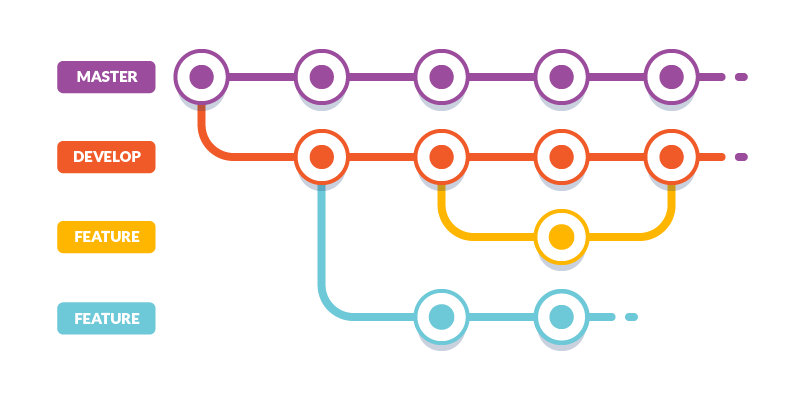
\includegraphics[width=\textwidth]{img/gitflow_workflow.png}
\caption{Illustration des GitFlow-Modells}
\label{fig:gitflow}
\end{figure*}

\paragraph{Beispielhafte Umsetzung in GitHub}

\begin{enumerate}
    \item Forke das Repository und erstelle einen neuen Branch: \texttt{git checkout -b feature/new-feature develop}
    \item Implementiere das neue Feature und pushe die Änderungen: \texttt{git push origin feature/new-feature}
    \item Öffne einen Pull Request von \texttt{feature/new-feature} nach \texttt{develop}.
    \item Die CI/CD-Pipeline führt die statische Code Analyse mit SonarQube durch.
    \item Bestehen alle Checks, kann der Branch gemerged werden.
\end{enumerate}

\paragraph{Screenshots und Ergebnisinterpretation}

Fügen Sie hier passende Screenshots ein, die die Ergebnisse der SonarQube-Analyse und den Workflow der GitHub Actions demonstrieren.

\begin{figure*}[h!]
\centering
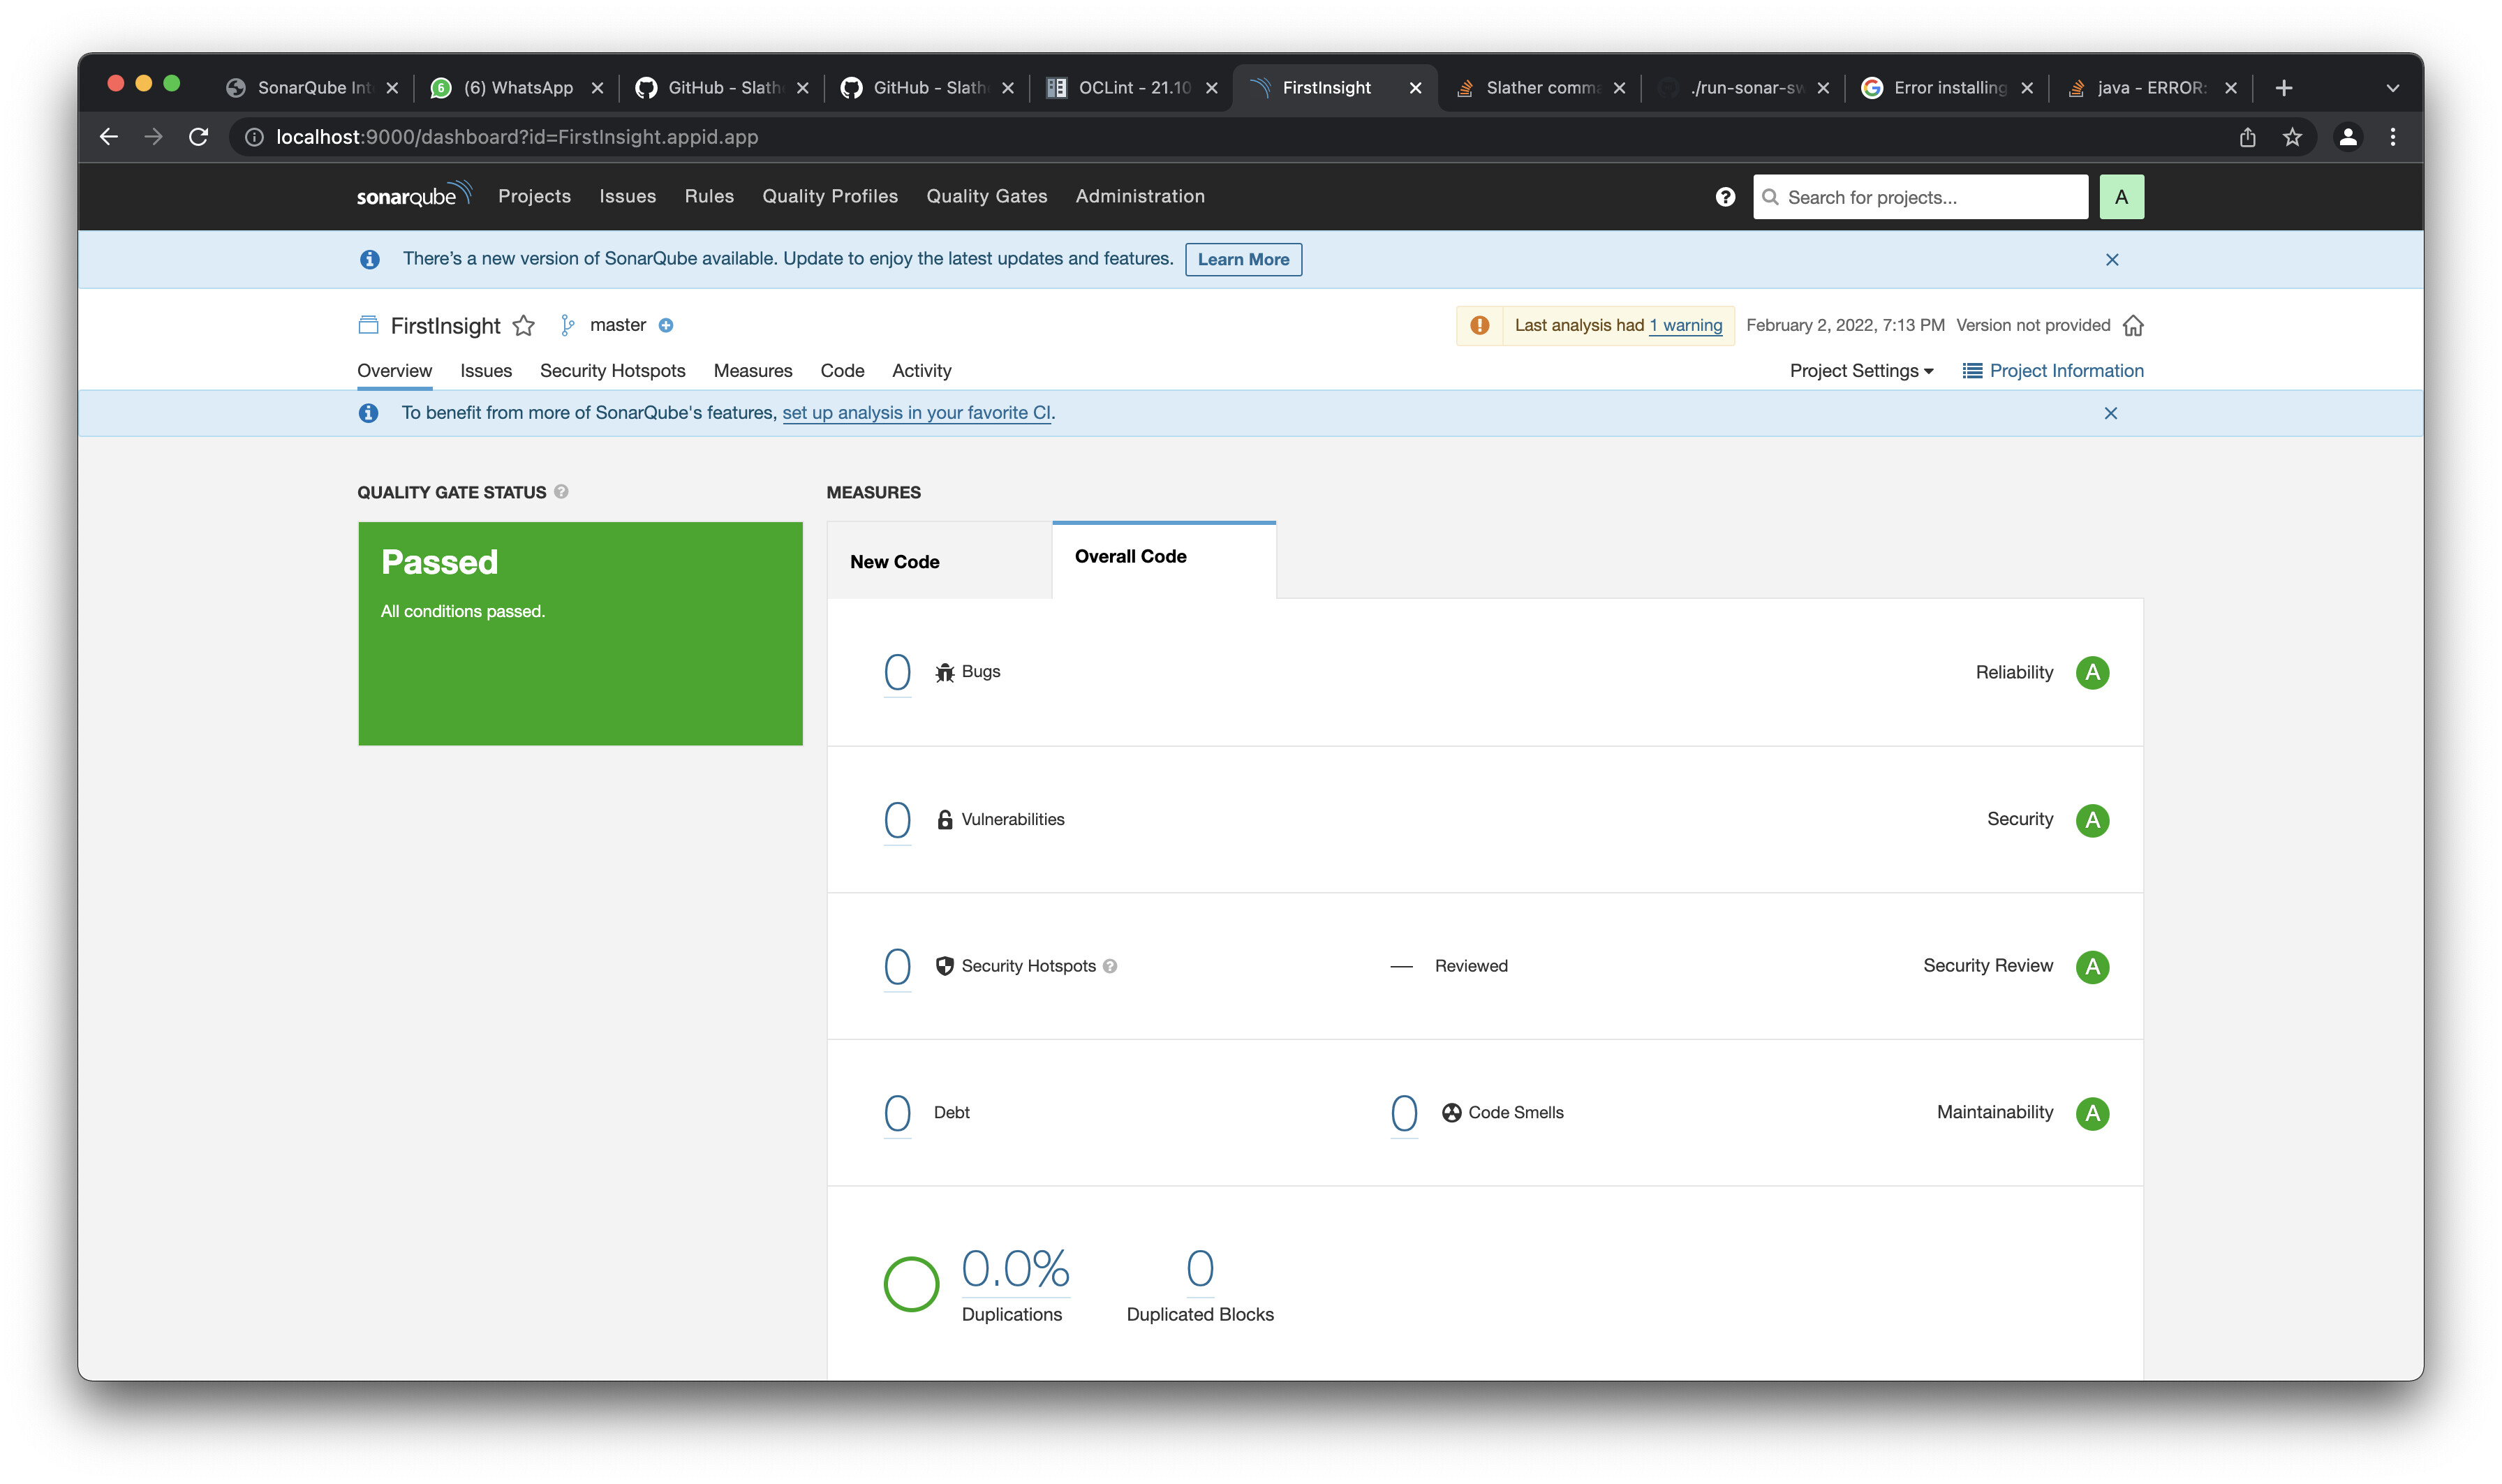
\includegraphics[width=\textwidth]{img/sonarqube_results.jpeg}
\caption{Ergebnisse der SonarQube-Analyse}
\label{fig:sonarqube_results}
\end{figure*}

\begin{figure*}[h!]
\centering
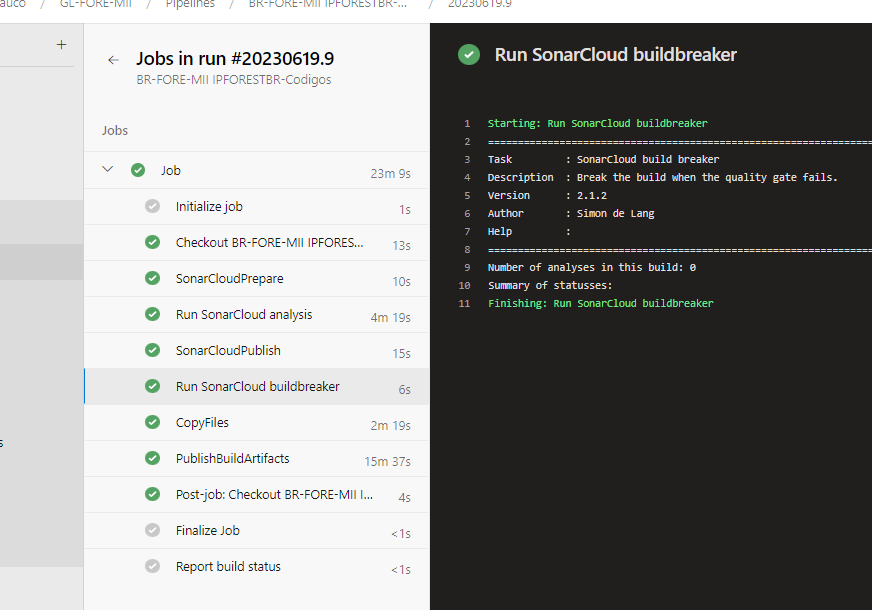
\includegraphics[width=\textwidth]{img/github_actions_failed_quality_gate.png}
\caption{GitHub Actions Workflow mit fehlgeschlagenem Quality Gate}
\label{fig:github_actions_failed_quality_gate}
\end{figure*}

\subsubsection{Metriken in SonarQube}

SonarQube bietet eine Vielzahl von Metriken, um die Qualität und Sicherheit des Codes zu bewerten. Zu den wichtigsten Metriken gehören:

\begin{itemize}
    \item \textbf{Bugs}: Fehler im Code, die potenziell zu falschem Verhalten führen.
    \item \textbf{Code Smells}: Hinweise auf Bereiche des Codes, die verbessert werden können.
    \item \textbf{Vulnerabilities}: Sicherheitslücken, die ausgenutzt werden könnten.
    \item \textbf{Coverage}: Prozentsatz des Codes, der durch Tests abgedeckt ist.
    \item \textbf{Duplications}: Anteil des Codes, der dupliziert ist.
\end{itemize}

\paragraph{Beispielhaftes SonarQube Dashboard}

\begin{figure*}[h!]
\centering
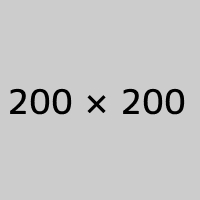
\includegraphics[width=\textwidth]{img/sonarqube_dashboard.png}
\caption{Beispiel eines SonarQube Dashboards}
\label{fig:sonarqube_dashboard}
\end{figure*}

\subsubsection{Schlussfolgerungen und Best Practices}

Die Integration von statischer Code Analyse in den CI/CD-Prozess verbessert nicht nur die Codequalität, sondern trägt auch zur Erhöhung der Sicherheit bei. Durch den Einsatz von Tools wie SonarQube in Kombination mit GitHub Actions, GitLab CI/CD oder Azure DevOps und strikten Branch-Regeln können potenzielle Schwachstellen frühzeitig erkannt und behoben werden.
